\chapter{Análisis técnico útil (y sus límites)}\label{cap:tecnico}

El análisis técnico tiene mala fama por las figuras subjetivas, pero algunas de sus herramientas son
simplemente \textbf{estadísticos del precio} que sirven para tres cosas concretas: identificar el
régimen (tendencia o rango), medir la volatilidad para colocar stops y definir niveles donde decidir.
Lo que \emph{no} hacen es predecir por sí solas.

\section{Tendencia: medias móviles}
La media simple $\text{SMA}_n(t) = \frac1n\sum_{k=0}^{n-1} P_{t-k}$ y la exponencial
$\text{EMA}_t = \alpha P_t + (1-\alpha)\text{EMA}_{t-1}$ con $\alpha = 2/(n+1)$
(\py{trader.indicators.sma}, \py{ema}). Un criterio de régimen muy usado:
\begin{itemize}
\item \textbf{Alcista}: precio $>$ SMA200 y SMA50 $>$ SMA200.
\item \textbf{Bajista}: precio $<$ SMA200 y SMA50 $<$ SMA200.
\item \textbf{Transición/rango}: el resto.
\end{itemize}
El \emph{momentum de series temporales} (estar largo si el precio está por encima de su media o si la
rentabilidad de 12 meses es positiva) es una de las anomalías mejor documentadas en todas las clases de
activo (Moskowitz, Ooi y Pedersen, 2012), aunque con largas rachas de bajo rendimiento.

\section{Osciladores}
\paragraph{RSI de Wilder.} $\text{RSI} = 100 - \dfrac{100}{1+RS}$ con $RS$ el cociente entre las
medias suavizadas (Wilder, $\alpha=1/n$) de subidas y bajadas. Valores extremos (RSI(2) $<10$) en una
acción en tendencia alcista son el ejemplo clásico de reversión a corto plazo
(\py{trader.backtest.rsi\_reversion}).

\paragraph{Bandas de Bollinger.} Media de 20 sesiones $\pm 2$ desviaciones típicas. \%B mide dónde
está el precio dentro de la banda. Un estrechamiento de bandas (\emph{squeeze}) indica baja
volatilidad, que tiende a ir seguida de expansión.

\paragraph{MACD.} Diferencia de EMA(12) y EMA(26), con señal EMA(9). Es un oscilador de tendencia.

\begin{figure}[h]\centering
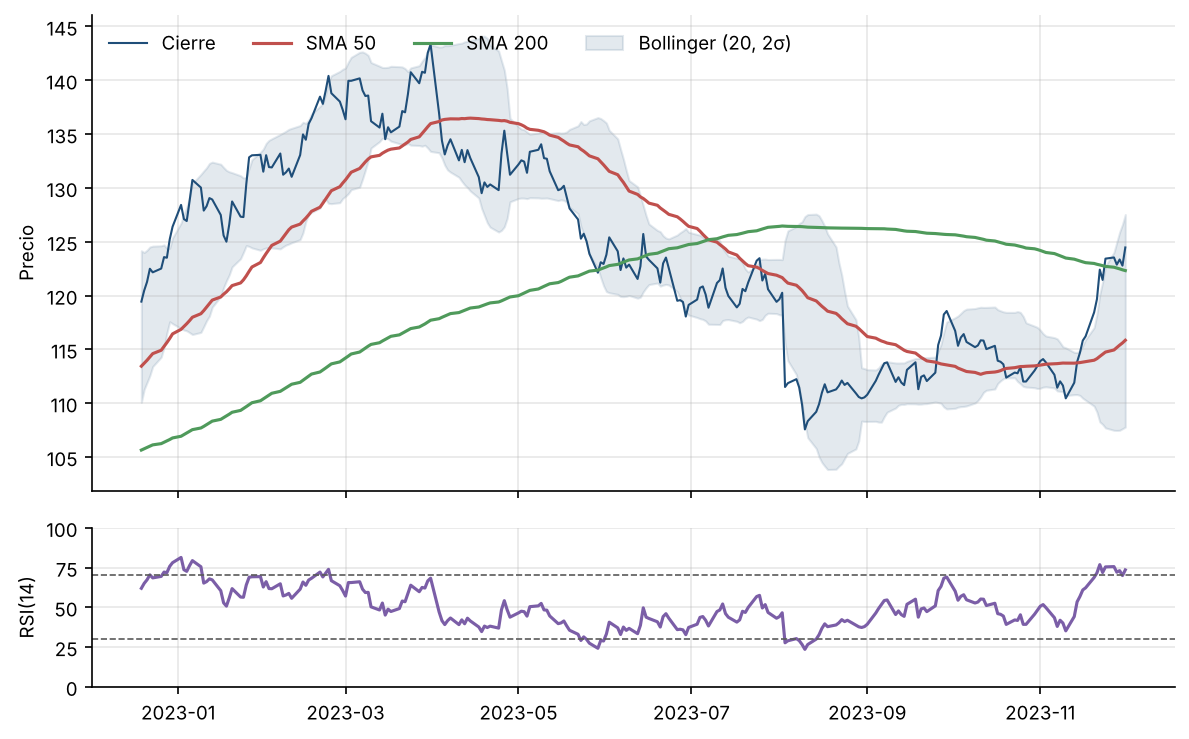
\includegraphics[width=\textwidth]{f01_indicadores}
\caption{Precio con SMA50, SMA200 y bandas de Bollinger; abajo, RSI(14) con los niveles 30/70.}
\end{figure}

\section{Volatilidad y stops: el ATR}
El rango verdadero $TR_t = \max(H_t-L_t,\ |H_t-C_{t-1}|,\ |L_t-C_{t-1}|)$ incluye los gaps; su media de
Wilder es el ATR. Colocar el stop a $k\cdot\text{ATR}$ ($k=1{,}5$--$3$) adapta la distancia al ruido del
activo y, combinado con el tamaño por riesgo (capítulo~\ref{cap:riesgo}), hace que cada operación
arriesgue lo mismo en dinero aunque los activos tengan volatilidades muy diferentes.

\section{Niveles}
\begin{itemize}
\item \textbf{Máximos y mínimos previos} (día, semana, 20 sesiones): donde se acumulan stops y órdenes.
\item \textbf{Canal de Donchian}: máximo y mínimo de las $n$ sesiones \emph{anteriores}. Romperlo es la
  base de los sistemas de seguimiento de tendencia tipo «tortuga» (\py{trader.backtest.donchian\_breakout}).
\item \textbf{Pivotes clásicos} (\py{trader.indicators.pivot\_points}) a partir del H, L, C de la sesión
  previa: $P=(H+L+C)/3$, $R_1=2P-L$, $S_1=2P-H$, $R_2=P+(H-L)$, $S_2=P-(H-L)$. Útiles intradía como
  referencias que mucha gente mira.
\item \textbf{VWAP} de la sesión: referencia de los algoritmos institucionales.
\end{itemize}

\begin{aviso}[El técnico no es una ventaja por sí mismo]
Cualquier regla técnica debe pasar por el proceso del capítulo~\ref{cap:backtest}. Un indicador sirve
para \emph{estructurar} la decisión (régimen, nivel, stop), no para sustituir una hipótesis de por qué
el precio debería moverse.
\end{aviso}

\begin{ejercicios}
\begin{enumerate}
\item Calcula los pivotes con $H=110$, $L=90$, $C=100$ y compáralos con la salida de \py{pivot\_points}.
\item Ejecuta \py{python scripts/backtest.py --estrategia rsi} y luego con \py{--estrategia sma}. ¿Cuál
  tiene más operaciones? ¿Cuál es más sensible a los costes (\py{--coste 5})?
\end{enumerate}
\end{ejercicios}
